
\section{Round 3: The Complete Mixer Atlas}
\label{sec:annex-experiment-3}

This annex reports Round~3 in full. Round~2 measured 868 configurations and left 194 of the 861 hybrid cells empty; Round~3 closes the matrix. The campaign trained every unordered pair of the $54$ registered mixers---$\binom{54}{2}=1{,}431$ cells, none missing---plus $54$ single-mixer baselines and $168$ ablation runs that move one switch at a time (optimizer family, normalization, positional encoding, Mixture-of-Experts routing, residual path, task and model class). It is the largest measurement in the project: $1{,}653$ training runs, $20.5$ million logged optimisation steps, and $3{,}668$ hours of training wall time spread over $7.2$ calendar days.

The annex follows the order of the analysis: the population and its caveats, the parameter landscape, the training outcomes, the learning dynamics, the gradient pressure per parameter block, the cost of training, the inference and quantization measurements, the reliability of the pipeline, and the correlations between the measured features. Every number is regenerated by \texttt{make\_report.py} from \texttt{master.csv}; every figure is regenerated by \texttt{make\_paper\_figures.py} from the same builders as the rest of the report, so this text and the artefacts cannot disagree.

\subsection{Setup, population and exclusions}

The harness produced $12{,}820$ stage records: $1{,}653$ training attempts, $4{,}686$ Transformers exports, $5{,}146$ inference evaluations, $1{,}334$ deploy records and one BitNet/GGUF conversion. Training succeeded $1{,}643$ times and failed $10$ times; the failures are ten \texttt{engram} pairs that exit with a non-zero code and are discussed in Section~\ref{sec:r3-reliability}. The population is summarised in Table~\ref{tab:r3-families}.

\begin{table}[H]
\centering
\small
\caption{Round~3 population by family: runs, median parameters, median final loss, wall hours per run, minutes per Mparam and training success rate.}
\label{tab:r3-families}
\begin{tabular}{lrrrrrrr}
\toprule
Family & $n$ & Smoke & Epochs & Params (M) & Final loss & min/Mparam & OK \\
\midrule
hybrid pairs & 1{,}431 & 22 & 459 & 0.32 & 8.778 & 421.5 & 99.3\% \\
single mixers & 54 & 0 & 382 & 0.26 & 8.998 & 546.5 & 100.0\% \\
optimizers & 39 & 0 & 312 & 0.31 & 9.321 & 311.5 & 100.0\% \\
text PE ablations & 12 & 1 & 370 & 0.31 & 8.826 & 297.2 & 100.0\% \\
ViT PE ablations & 39 & 0 & 499 & 0.35 & 1.004 & 207.8 & 100.0\% \\
vision tasks & 9 & 0 & 499 & 0.34 & 1.004 & 244.3 & 100.0\% \\
audio tasks & 4 & 1 & 499 & 0.45 & 1.098 & 23.6 & 100.0\% \\
real-data runs & 8 & 0 & 499 & 0.33 & 1.099 & 84.9 & 100.0\% \\
tokenizers & 4 & 0 & 499 & 0.31 & 6.130 & 31.5 & 100.0\% \\
architecture switches & 23 & 4 & 370 & 0.31 & 8.942 & 318.1 & 100.0\% \\
MoE variants & 17 & 15 & 499 & 0.37 & 8.873 & 556.3 & 100.0\% \\
normalization & 6 & 0 & 312 & 0.31 & 8.944 & 237.0 & 100.0\% \\
batch size & 2 & 0 & 406 & 0.31 & 8.669 & 238.1 & 100.0\% \\
task switches & 4 & 0 & 499 & 0.31 & 6.426 & 265.0 & 100.0\% \\
\bottomrule
\end{tabular}
\end{table}

Two exclusions shape the rest of the annex. First, the \emph{deployment} stage is not analysed. In this round the deployer received the live \texttt{FrankensteinModelConfig} dataclass stored in the checkpoint where it expected a mapping and called \texttt{.get()} on it, so $822$ of the $1{,}334$ deploy records failed with \texttt{'FrankensteinModelConfig' object has no attribute 'get'}. Measuring a broken stage would confound a serialisation bug with quantization quality; the deployment path is therefore dropped, and the analysis of quantized weights uses the Transformers-export path instead, which exported $4{,}686$ models with no failures. Second, only $662$ of the training runs produced Hugging Face inference rows ($33{,}380$ sample rows over $653$ MLM pairs plus a handful of causal-LM and text-classification runs); the inference section is a study of that subset, not of the whole atlas.

The runs are heterogeneous in a way that matters for the curves. The configurations ask for 500 epochs, but the harness stops a run earlier (by schedule, plateau criterion or an ablation-specific cap): $734$ runs reached the last epoch and $919$ stopped earlier. The learning curves are therefore stretched over each run's own progress instead of being plotted against absolute steps, so a 300-epoch run and a 500-epoch run can be compared at the same fraction of their schedule. The throughput and cost analysis keeps absolute times, because that is what the campaign paid. The 61 runs with fewer than 5{,}000 logged steps are dominated by the audio, tokenizer and real-data families, whose datasets are small enough to finish in seconds. A stronger distinction matters for every comparison that follows: $44$ runs stopped before epoch~100---fifteen of the seventeen MoE ablations (five-epoch routing smoke tests), the single BitNet/GGUF conversion and a dozen truncated hybrid pairs. They stay in the population and in the compute ledger, but every loss, dynamics, gradient, cost-per-run and correlation result is computed on the $1{,}609$ runs with at least 100 epochs. The budget column of Table~\ref{tab:r3-families} makes the distinction visible.

\begin{figure}[tbp]
\centering
\fitfigure{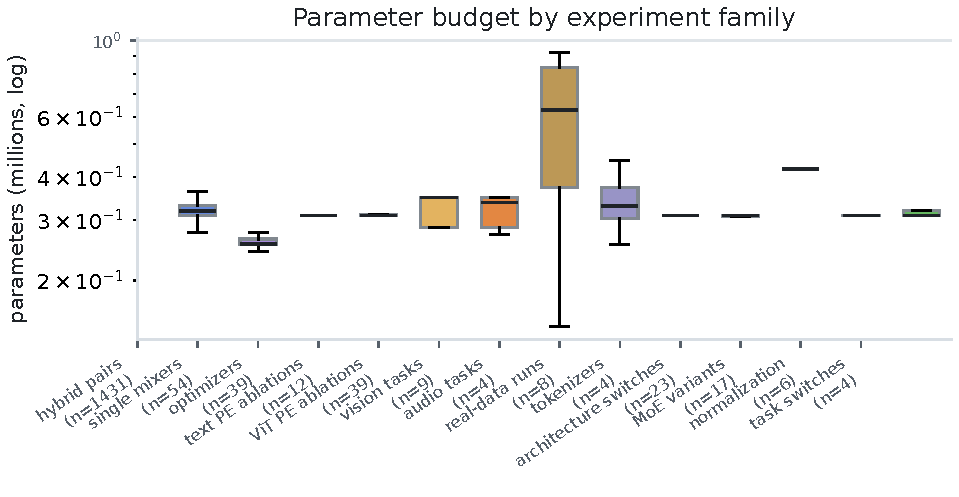
\includegraphics{figures/experiments/round3/params_family_box.pdf}}
\caption{Parameter budget by experiment family (log scale).}
\label{fig:r3-params-family}
\end{figure}
\begin{figure}[tbp]
\centering
\fitfigure{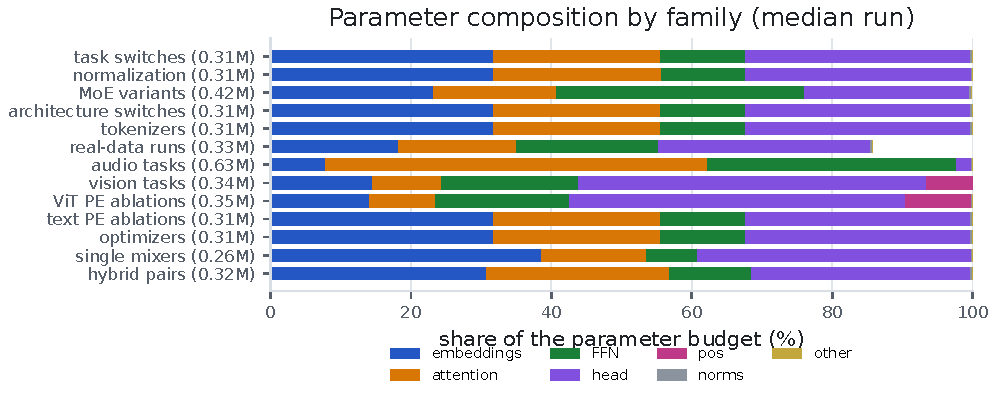
\includegraphics{figures/experiments/round3/params_composition.pdf}}
\caption{Where the parameters live, by family. Embeddings and the head are fixed costs; attention and the FFN carry the architectural differences.}
\label{fig:r3-params-composition}
\end{figure}

\subsection{The parameter landscape}

The $1{,}653$ runs span $147{,}171$ to $1{,}957{,}440$ parameters (median $315{,}744$). The median run sits at $315{,}744$ parameters and the median hybrid pair at $318{,}784$, with a composition that is almost independent of the family: the token embedding and the output head are fixed costs of roughly $31.0\%$ and $31.6\%$ of the budget, attention takes $24.8\%$, the FFN $11.8\%$ and the normalization layers $0.3\%$. The architectural choice therefore moves a quarter of the parameters; the other three quarters are the price of having a vocabulary and a classifier. Vision transformers are the exception: patch embeddings replace the token embedding and the classification head is small, so their budget is dominated by attention and FFN.

Parameter cost has a clear per-mixer reading, and it is not the reading one would guess from the literature. The cheapest second mixers are \texttt{mamba} (0.28M), \texttt{ccgqa} (0.29M), \texttt{cca} (0.29M); the most expensive are \texttt{gmla} (1.67M), \texttt{engram} (0.60M), \texttt{mfa} (0.54M). \texttt{engram} pays for its key--value memory bank, and \texttt{gmla} pays for the latent projections of the gated multi-head latent attention. Cheapness does not predict quality: \texttt{ccgqa} and \texttt{gqa} are among the cheapest and end slightly below the pair median, while \texttt{mamba}, \texttt{cca} and \texttt{mlra} are equally cheap and end above it; \texttt{engram} buys 0.28M extra parameters for a loss indistinguishable from the median.

The scatter of final loss against parameter count (Figure~\ref{fig:r3-params-loss}) has a rank correlation of $-0.42$ over the $1{,}431$ pairs: larger models are somewhat better, but size explains only a sixth of the ranking, and the atlas spans more than a factor of ten in size against two nats of loss. The budget helps; it does not decide. This is the same conclusion as Round~2, now measured on the complete grid rather than on two thirds of it.

\begin{figure}[tbp]
\centering
\fitfigure{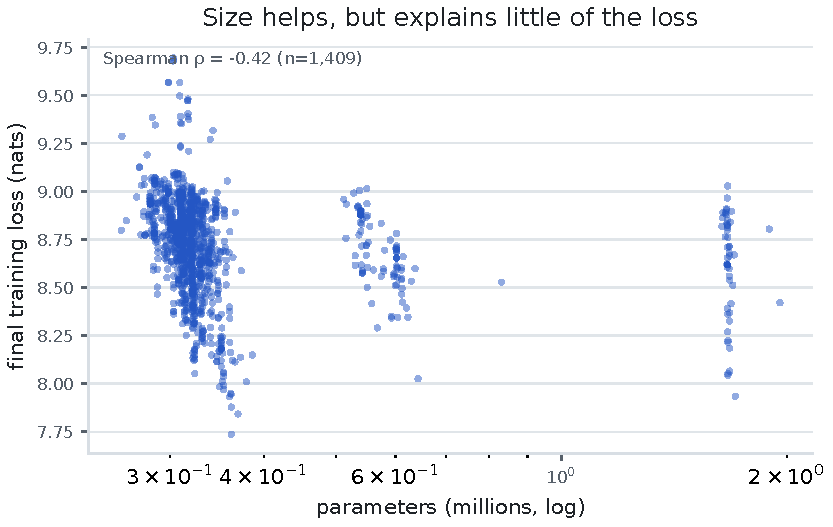
\includegraphics{figures/experiments/round3/params_vs_loss.pdf}}
\caption{Final training loss against parameter count for the hybrid pairs.}
\label{fig:r3-params-loss}
\end{figure}

\subsection{Training outcomes}

The hybrid pairs end at a median final loss of $8.78$ nats (from $7.74$ to $9.70$), the best being $\texttt{attn\_falcon2a\_\_conformer}$ at $7.736$ and the worst $\texttt{attn\_mtla\_\_tpa}$ at $9.70$. Table~\ref{tab:r3-top-loss} lists the ten best pairs. The spread is wide: the difference between the best and the worst pair is larger than the difference between the best and the median optimizer, normalization or positional-encoding ablation. The mixer stack is the dominant design decision of the round, exactly as in Round~2.

\begin{table}[H]
\centering
\small
\caption{The ten best hybrid pairs by final training loss.}
\label{tab:r3-top-loss}
\begin{tabular}{rlrrr}
\toprule
\# & Pair & Params (M) & Final loss & Hours \\
\midrule
1 & \texttt{attn\_falcon2a\_\_conformer} & 0.36 & 7.736 & 2.75 \\
2 & \texttt{attn\_hgrn2\_\_conformer} & 0.37 & 7.842 & 1.87 \\
3 & \texttt{attn\_falcon2\_\_conformer} & 0.36 & 7.878 & 2.88 \\
4 & \texttt{attn\_nsa\_\_conformer} & 0.36 & 7.931 & 2.72 \\
5 & \texttt{attn\_conformer\_\_gmla} & 1.71 & 7.934 & 3.51 \\
6 & \texttt{attn\_gated\_deltanet\_\_conformer} & 0.36 & 7.945 & 2.88 \\
7 & \texttt{attn\_kda\_\_conformer} & 0.36 & 7.948 & 2.30 \\
8 & \texttt{attn\_falcon1a\_\_conformer} & 0.35 & 7.969 & 2.73 \\
9 & \texttt{attn\_gated\_deltanet2\_\_falcon2a} & 0.35 & 7.984 & 2.36 \\
10 & \texttt{attn\_falcon3a\_\_conformer} & 0.35 & 7.991 & 2.83 \\
\bottomrule
\end{tabular}
\end{table}
\begin{figure}[tbp]
\centering
\fitfigure{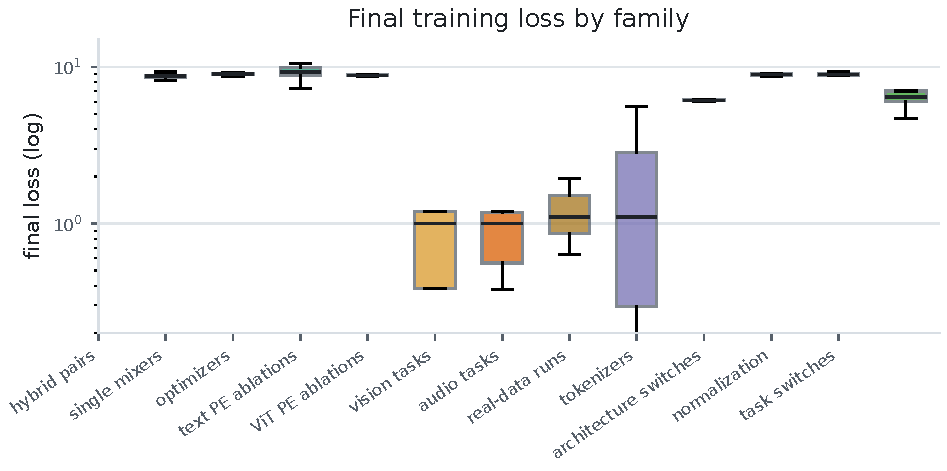
\includegraphics{figures/experiments/round3/loss_family_box.pdf}}
\caption{Final training loss by family. Tasks are not comparable across families; the log axis keeps them visible.}
\label{fig:r3-loss-family}
\end{figure}

Loss is not comparable across families because the task changes: the MLM families sit at 8.8--9.3 nats, the vision families at about 1.0, the audio and real-data families at about 1.0 (cross-entropy over a different label space), and the tokenizer runs at 6.0. Figure~\ref{fig:r3-loss-family} keeps them on a log axis for that reason. The MoE ablations need the budget caveat: the fifteen five-epoch routing variants never leave the first epoch and are excluded, so only the two full-schedule variants---\texttt{moe\_interleaved} and \texttt{moe\_latent}---are comparable with the pair population, where they land at the pair median. The routing study is therefore a smoke test in this round and not evidence about expert capacity.

Held-out quality is measured by the inference rows. Across the $653$ MLM pairs the mean top-1 accuracy is $4.46\%$ and the mean top-5 hit rate is $24.0\%$; the medians are 0 and 28.6\%, so the distribution is a mixture of a few pairs that learned something and a majority that did not. Table~\ref{tab:r3-top-inference} lists the best pairs. The rank correlation between final training loss and held-out top-5 is only $+0.14$, so a lower training loss does not imply a better model at this scale---the same warning as in Round~2, now on 653 pairs instead of 667.

\begin{table}[H]
\centering
\small
\caption{The ten best pairs by held-out top-5 hit rate (unquantized export).}
\label{tab:r3-top-inference}
\begin{tabular}{rlrrr}
\toprule
\# & Pair & Top-1 & Top-5 & Final loss \\
\midrule
1 & \texttt{attn\_bigbird\_\_ccgqa} & 0.00\% & 42.9\% & 8.784 \\
2 & \texttt{attn\_bigbird\_\_sparsek} & 0.00\% & 42.9\% & 8.649 \\
3 & \texttt{attn\_bigbird\_\_ssog} & 0.00\% & 42.9\% & 8.732 \\
4 & \texttt{attn\_cca\_\_gmla} & 0.00\% & 42.9\% & 8.889 \\
5 & \texttt{attn\_cca\_\_kda} & 0.00\% & 42.9\% & 8.718 \\
6 & \texttt{attn\_ccgqa\_\_ca} & 14.29\% & 42.9\% & 8.764 \\
7 & \texttt{attn\_ccgqa\_\_falcon2} & 14.29\% & 42.9\% & 8.656 \\
8 & \texttt{attn\_ccgqa\_\_falcon2a} & 14.29\% & 42.9\% & 8.551 \\
9 & \texttt{attn\_ccgqa\_\_fastconformer} & 14.29\% & 42.9\% & 8.761 \\
10 & \texttt{attn\_ccgqa\_\_kpa} & 14.29\% & 42.9\% & 8.963 \\
\bottomrule
\end{tabular}
\end{table}

\subsection{Learning dynamics}

Figure~\ref{fig:r3-curves-quantiles} shows the population curve. The median pair starts at $10.50$ nats and ends at $8.78$; the P10--P90 band at the end is $8.41$--$8.97$, narrower than the spread between families. Most of the reduction happens in the first quarter: the median reaches $9.47$ at 25\% of the schedule, $8.92$ at half and $8.75$ at three quarters. Round~3 therefore measures how fast a configuration learns, not where it converges: the curves are still descending when the schedule ends.

\begin{figure}[tbp]
\centering
\fitfigure{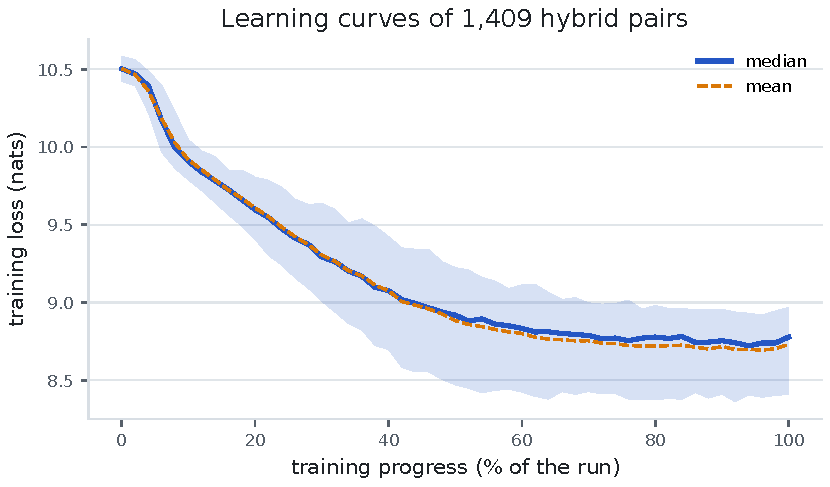
\includegraphics{figures/experiments/round3/curves_quantiles.pdf}}
\caption{Population learning curves with a P10--P90 band, normalised to each run's own schedule.}
\label{fig:r3-curves-quantiles}
\end{figure}
\begin{figure}[tbp]
\centering
\fitfigure{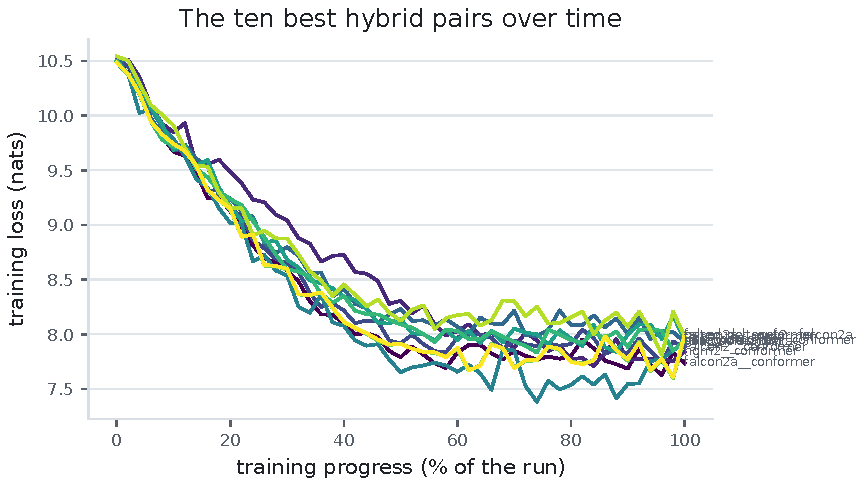
\includegraphics{figures/experiments/round3/curves_top10.pdf}}
\caption{The ten best hybrid pairs over their own training schedule.}
\label{fig:r3-curves-top10}
\end{figure}

The ordering of the best pairs is established early. By a quarter of the schedule the per-pair loss already ranks the pairs with a Spearman correlation of $0.62$ against their final ordering, and in Figure~\ref{fig:r3-curves-top10} the ten best separate from the population before the halfway mark and rarely cross afterwards. The number of epochs needed to reach 90\% of a run's total loss drop confirms this: the median is $41\%$ of the schedule, and the family medians range from $21\%$ for the vision tasks (where the loss collapses almost immediately) to $56\%$ for the normalization ablations (where the differences between norms only appear late). Hybrid pairs sit at $40\%$.

\begin{figure}[tbp]
\centering
\fitfigure{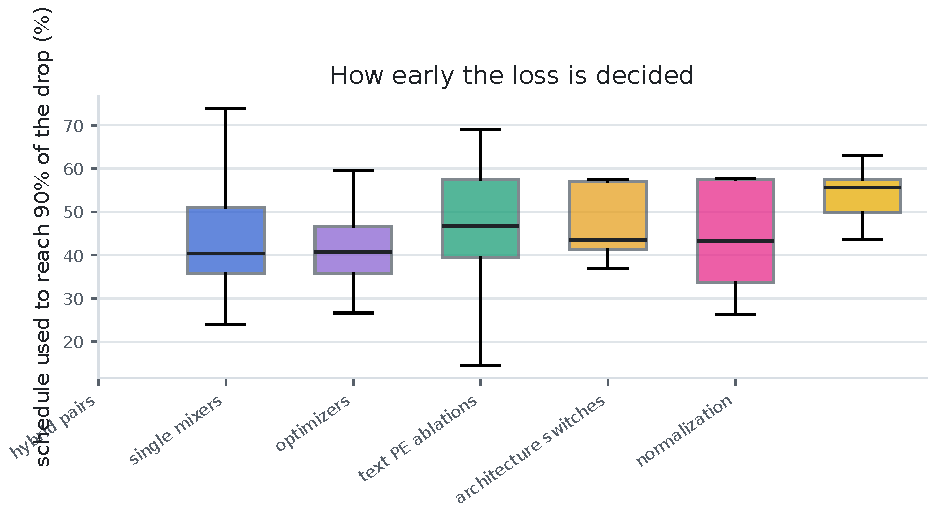
\includegraphics{figures/experiments/round3/convergence_speed.pdf}}
\caption{Fraction of the schedule needed to reach 90\% of a run's total loss drop, by family.}
\label{fig:r3-convergence}
\end{figure}

\subsection{Gradient pressure per parameter block}

The trainer logs the L2 norm of the gradient of every parameter block after clipping: embeddings, positional encoding, attention, FFN, normalization, head, mHC, router, residual and other. Table~\ref{tab:r3-gradients} reproduces the medians and Figure~\ref{fig:r3-grad-groups} the trajectories over training.

\begin{table}[H]
\centering
\small
\caption{Gradient norm per parameter block: median of the per-run mean, median of the last step, coefficient of variation and share of runs where the block is active.}
\label{tab:r3-gradients}
\begin{tabular}{lrrrr}
\toprule
Block & Mean & Final & CV & Active \\
\midrule
embeddings & 0.152 & 0.163 & 0.27 & 99.9\% \\
positional & 0.000 & 0.000 & 1.79 & 3.5\% \\
attention & 2.121 & 2.503 & 0.22 & 100.0\% \\
FFN & 0.709 & 0.674 & 0.31 & 100.0\% \\
norms & 0.326 & 0.336 & 0.13 & 99.9\% \\
head & 3.657 & 3.733 & 0.13 & 100.0\% \\
mHC & 0.000 & 0.000 & 0.03 & 0.1\% \\
router & 0.000 & 0.000 & 0.50 & 1.2\% \\
residual & 0.000 & 0.000 & 0.82 & 0.1\% \\
other & 0.000 & 0.000 & n/a & 0.0\% \\
\bottomrule
\end{tabular}
\end{table}
\begin{figure}[tbp]
\centering
\fitfigure{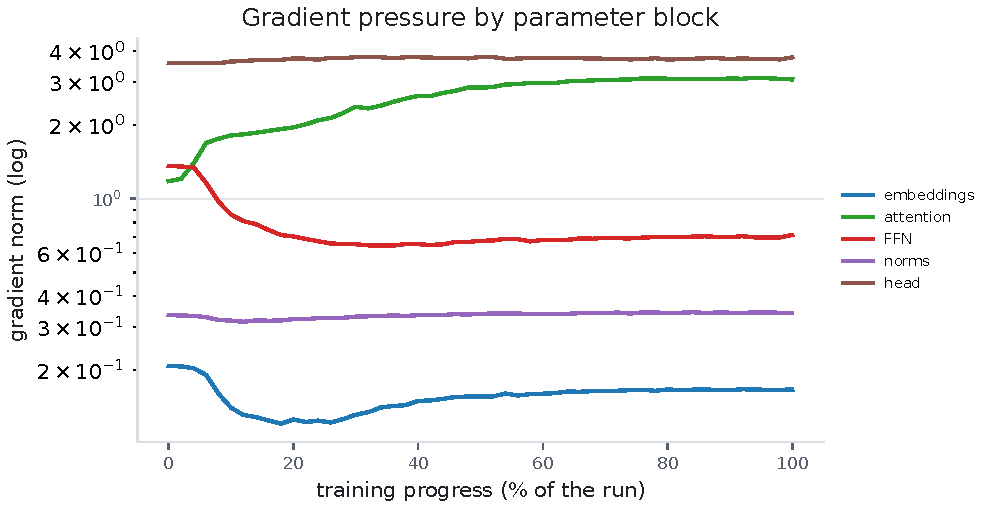
\includegraphics{figures/experiments/round3/grad_groups_curves.pdf}}
\caption{Median gradient norm per parameter block over training (post-clip).}
\label{fig:r3-grad-groups}
\end{figure}

Three facts stand out. First, the head carries the largest gradient ($3.66$ on average, $3.73$ at the end), followed by attention ($2.12$, $2.50$) and the FFN ($0.71$, $0.67$); embeddings and normalization are an order of magnitude smaller ($0.15$ and $0.33$). The ordering is stable across the whole campaign, which is why the per-block normalization of the optimizer groups is not a cosmetic choice. Second, the coefficients of variation are small---$0.13$ for the head, $0.22$ for attention, $0.31$ for the FFN---so the gradient scale of a block is a property of the architecture, not of the step. Third, the blocks that only exist in some configurations (\texttt{mhc}, \texttt{router}, \texttt{residual}) are exactly zero in the runs that do not enable them, which is what makes the zero-median rows of the table meaningful rather than missing data.

\begin{figure}[tbp]
\centering
\fitfigure{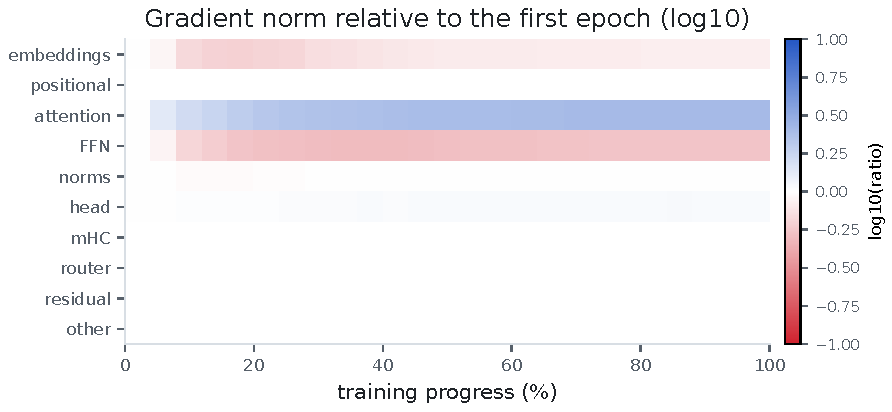
\includegraphics{figures/experiments/round3/grad_heatmap.pdf}}
\caption{Gradient norm per block relative to its first epoch, in log10 units.}
\label{fig:r3-grad-heatmap}
\end{figure}

The heatmap (Figure~\ref{fig:r3-grad-heatmap}) reads the same statistics as a function of progress. The head is flat, attention grows slightly, and the FFN decays by a factor of about two over the first half of training before stabilizing; the embeddings decay as the vocabulary statistics are learned. Nothing explodes: there are no NaN steps in the whole campaign, $109$ Inf steps (all repaired in place, in $15$ runs), and the gradient-norm coefficient of variation is inversely related to the final loss ($-0.61$), i.e.\ the runs that end lower have slightly more variable gradients, not less.

\begin{figure}[tbp]
\centering
\fitfigure{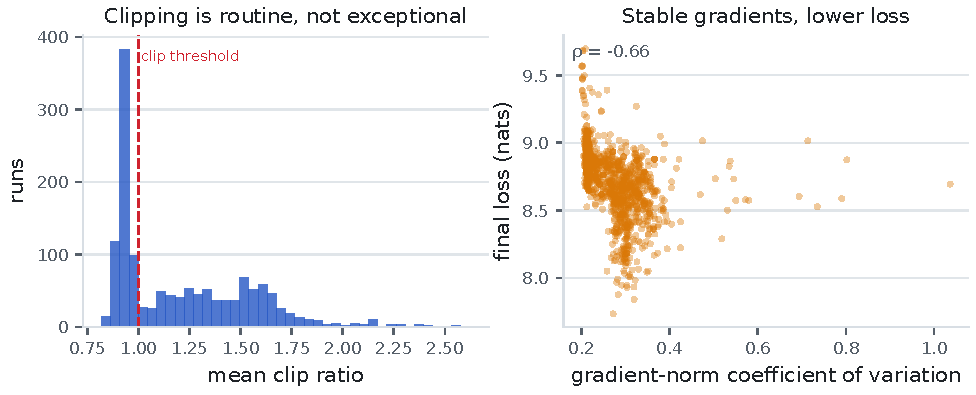
\includegraphics{figures/experiments/round3/grad_health.pdf}}
\caption{Clip ratio distribution and gradient variability against final loss.}
\label{fig:r3-grad-health}
\end{figure}

Clipping, however, is routine rather than exceptional. The median mean clip ratio is $1.04$---just above the threshold of 1---and $51.6\%$ of the runs spend the campaign clipping on average, with a P90 of $1.65$. Round~2 reported a median of 0.90 and clipping as a rare event; the difference is the longer schedule and the higher learning rates of Round~3. The consequence for the report is that gradient norms should be read as post-clip norms, which is what the trainer logs.

The memory footprint is modest: the median run peaks at $1{,}457$ MB of resident memory and the maximum is $3{,}159$ MB, so the whole atlas fits on a single CPU host with a dozen workers.

\subsection{Throughput and cost}

Training time grows only weakly with parameters: a log-log fit over the MLM pairs gives an exponent of $0.25$ with $R^2=0.06$. The reason is that the parameter count is not what the clock measures---the number of steps dominates, and the step count varies by family and by early stopping. The normalised cost (Figure~\ref{fig:r3-cost-mparam}) is the quantity that compares architectures fairly: the median run spends $402$ minutes per million parameters, and the family medians span a factor of about three around that value. A hybrid pair costs $422$ minutes per Mparam, slightly below a single-mixer baseline ($547$) and above an optimizer ablation ($311$); the differences come from the effective schedule and from the update cost, not from the parameter count.

\begin{figure}[tbp]
\centering
\fitfigure{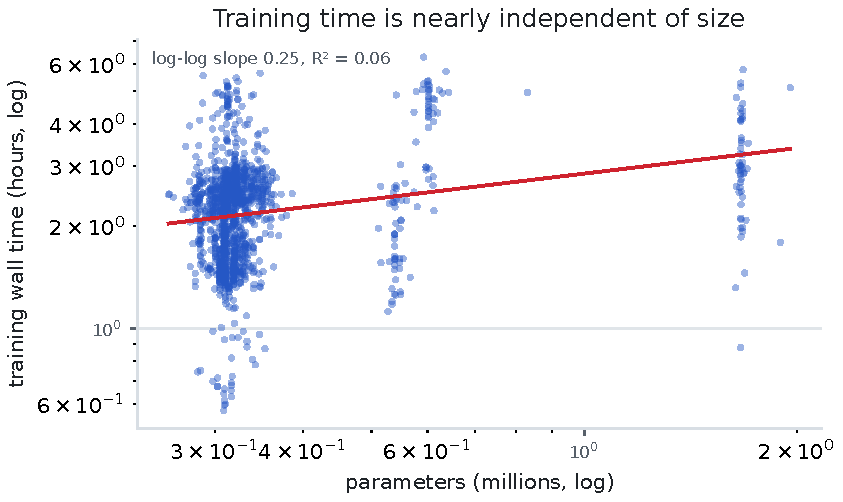
\includegraphics{figures/experiments/round3/time_vs_params.pdf}}
\caption{Training wall time against parameter count, with the log-log fit.}
\label{fig:r3-time-params}
\end{figure}
\begin{figure}[tbp]
\centering
\fitfigure{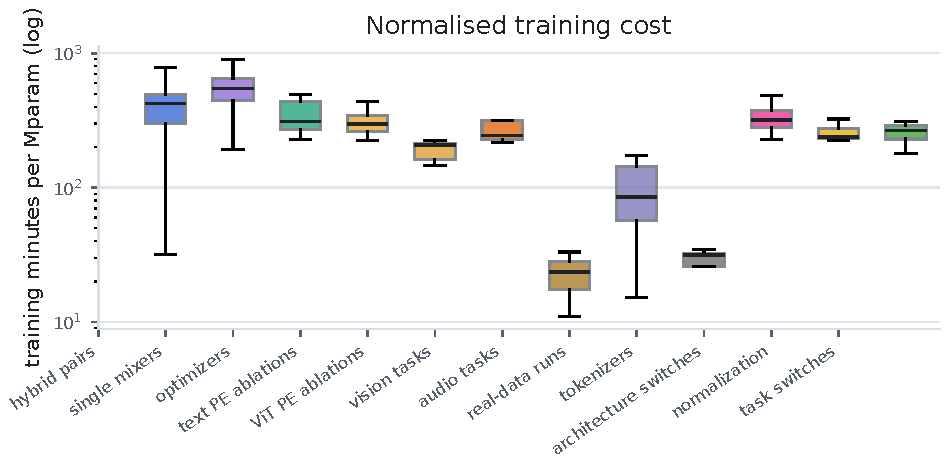
\includegraphics{figures/experiments/round3/cost_per_mparam.pdf}}
\caption{Training minutes per million parameters, by family.}
\label{fig:r3-cost-mparam}
\end{figure}
\begin{figure}[tbp]
\centering
\fitfigure{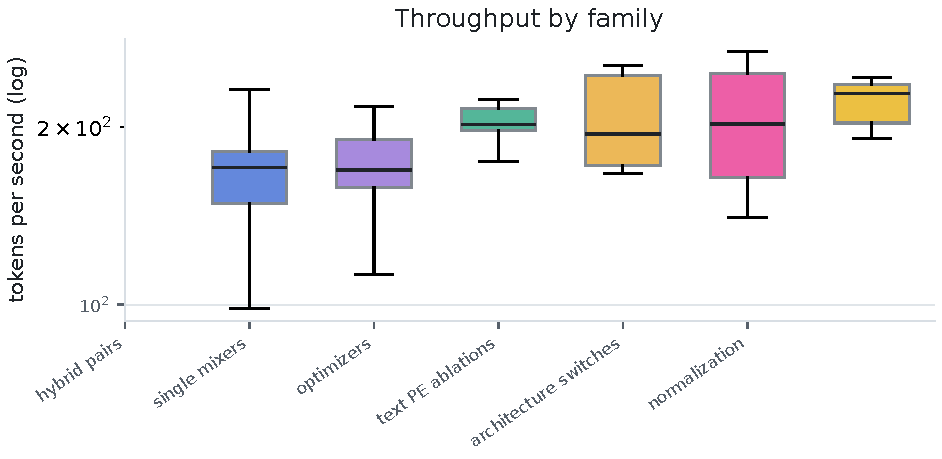
\includegraphics{figures/experiments/round3/throughput_family.pdf}}
\caption{Logging throughput by family (tokens per second, log scale).}
\label{fig:r3-throughput}
\end{figure}
\begin{figure}[tbp]
\centering
\fitfigure{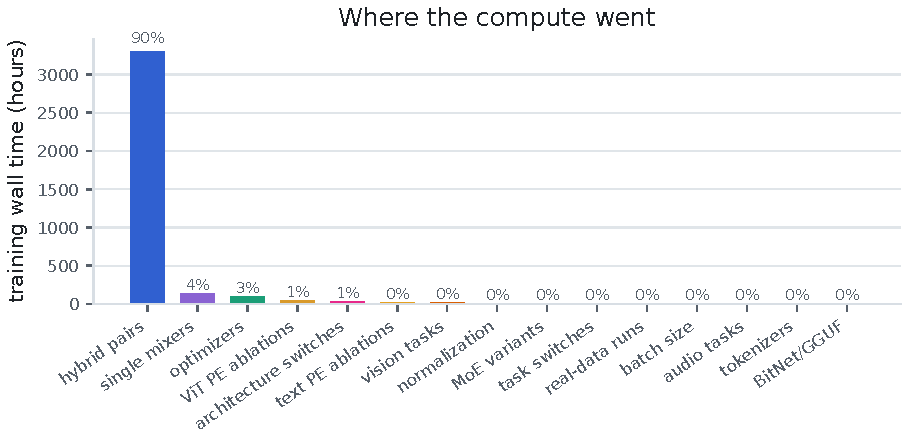
\includegraphics{figures/experiments/round3/compute_by_family.pdf}}
\caption{Share of the training wall time by family.}
\label{fig:r3-compute}
\end{figure}

Figure~\ref{fig:r3-compute} shows where the $3{,}668$ hours went. The hybrid pairs consume $90.0\%$ of the campaign ($3{,}301$ hours), the single-mixer baselines $3.6\%$ and every other family less than 3\%. The vision and audio families are cheap in wall time despite their long schedules because their steps are short; the throughput panel (Figure~\ref{fig:r3-throughput}) makes the same point in tokens per second: the MLM pairs run at a median of $171$ tokens/s, while the vision family is an order of magnitude slower ($14.3$ tokens/s) because its inputs are images rather than 64-token sequences.

The campaign spent $3{,}668$ hours of training wall time spread over $7.2$ calendar days with 13--26 workers, which is the parallel efficiency of the harness rather than a property of the models.

\subsection{Inference and quantization}

The inference section studies the $662$ runs that produced Hugging Face rows: $653$ MLM pairs, four causal-LM runs and one text-classification run. Each run was exported unquantized (\texttt{hf\_none}) and re-exported with three codecs at two loader runtimes (\texttt{q8\_0}, \texttt{q4\_0}, \texttt{i2\_s}, each in \texttt{v1} and \texttt{v2}). The two runtimes sampled different mask positions---only 3.5\% of the \texttt{v1} sample keys coincide with the baseline---so \texttt{v1} cannot be paired with \texttt{hf\_none}; the clean comparison is the \texttt{v2} family, which reuses the baseline masks for 99.4\% of the keys. This is a property of the harness, not of the models, and it is the main caveat of the section.

\begin{figure}[tbp]
\centering
\fitfigure{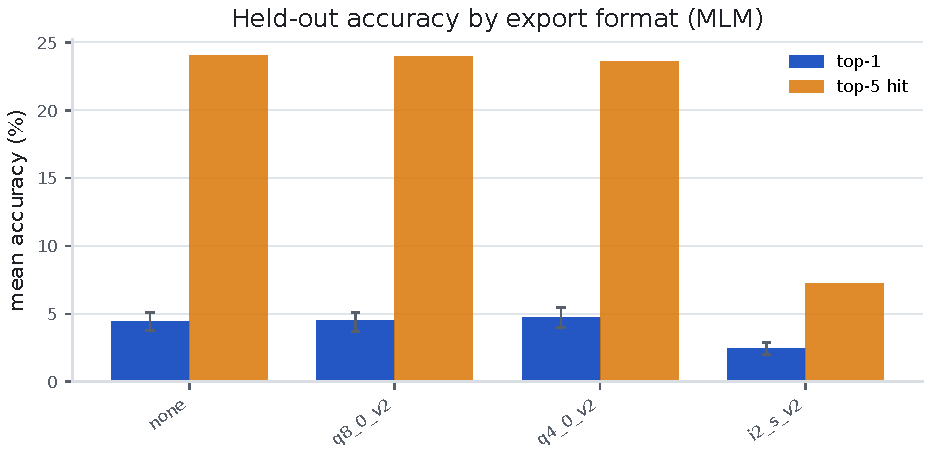
\includegraphics{figures/experiments/round3/inference_format_accuracy.pdf}}
\caption{Held-out top-1 and top-5 accuracy of the unquantized export and the three v2 codecs.}
\label{fig:r3-inference-format}
\end{figure}

The aggregate view (Figure~\ref{fig:r3-inference-format} and Table~\ref{tab:r3-formats}) says that 8-bit and 4-bit weights are essentially free at this scale. Relative to the unquantized export, \texttt{q8\_0\_v2} changes the top-1 accuracy by $+0.07$ percentage points and leaves $99.2\%$ of the pairs unchanged, with only $0.2\%$ degrading; \texttt{q4\_0\_v2} changes it by $+0.33$ points with $94.5\%$ unchanged and $1.7\%$ degrading. The 2-bit codec is the exception: \texttt{i2\_s\_v2} changes the top-1 accuracy by $-2.03$ points on average, leaves $73.2\%$ of the pairs intact and degrades $18.7\%$ of them. The \texttt{v1} rows are shown in the table for completeness but are not comparable with the baseline, because their masks are harder: the same pairs score $14.4\%$ top-5 under \texttt{v1} against $24.0\%$ under \texttt{hf\_none}.

\begin{table}[H]
\centering
\small
\caption{Held-out accuracy per export format (MLM): evaluated pairs, mean top-1 and top-5, mean delta against the unquantized export, 95\% bootstrap interval and share of pairs that degrade.}
\label{tab:r3-formats}
\begin{tabular}{lrrrcrr}
\toprule
Format & $n$ & Top-1 & Top-5 & $\Delta$ (pp) & 95\% CI & Worse \\
\midrule
none & 653 & 4.46 & 24.0 & 0.000 & -- & 0.0\% \\
\texttt{q8\_0\_v1} & 653 & 2.87 & 14.4 & -1.663 & -2.406 / -0.788 & 22.2\% \\
\texttt{q8\_0\_v2} & 653 & 4.50 & 23.9 & +0.066 & -0.022 / +0.175 & 0.2\% \\
\texttt{q4\_0\_v1} & 653 & 2.72 & 14.1 & -1.816 & -2.560 / -0.919 & 22.2\% \\
\texttt{q4\_0\_v2} & 653 & 4.76 & 23.6 & +0.328 & +0.088 / +0.569 & 1.7\% \\
\texttt{i2\_s\_v1} & 653 & 0.83 & 3.2 & -3.719 & -4.375 / -3.040 & 24.2\% \\
\texttt{i2\_s\_v2} & 653 & 2.41 & 7.2 & -2.035 & -2.713 / -1.313 & 18.7\% \\
\bottomrule
\end{tabular}
\end{table}

The sample-level view is sharper than the aggregate. Matching each quantized prediction to the baseline prediction of the same mask, \texttt{q8\_0\_v2} agrees on $99.5\%$ of the samples (95\% CI from the per-combo bootstrap), \texttt{q4\_0\_v2} on $91.8\%$ and \texttt{i2\_s\_v2} on only $20.8\%$. The 2-bit model is not a slightly worse copy of the teacher: it is a different model that happens to preserve the aggregate top-1 on the pairs whose baseline accuracy was already near zero.

\begin{figure}[tbp]
\centering
\fitfigure{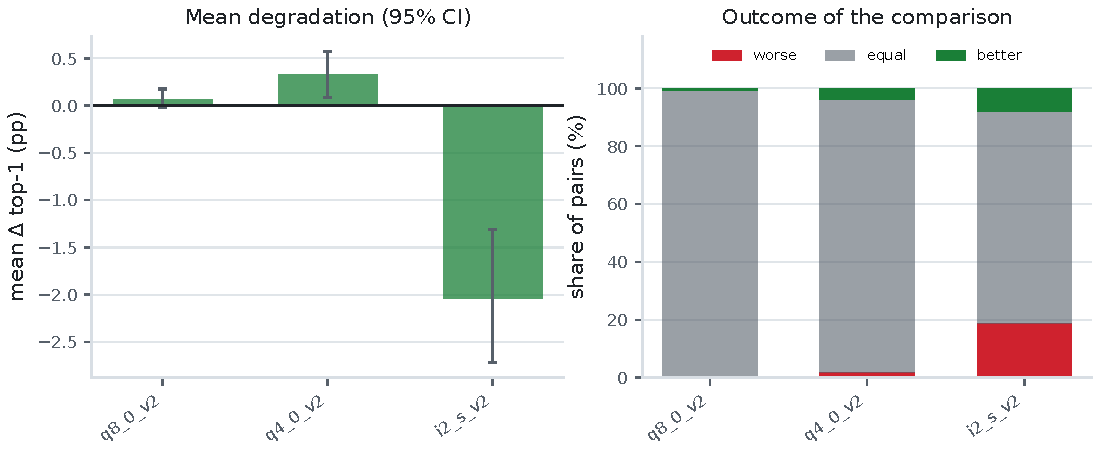
\includegraphics{figures/experiments/round3/quant_delta_dist.pdf}}
\caption{Mean top-1 delta against the unquantized export (95\% bootstrap CI) and the share of pairs that degrade, stay equal or improve.}
\label{fig:r3-quant-delta}
\end{figure}
\begin{figure}[tbp]
\centering
\fitfigure{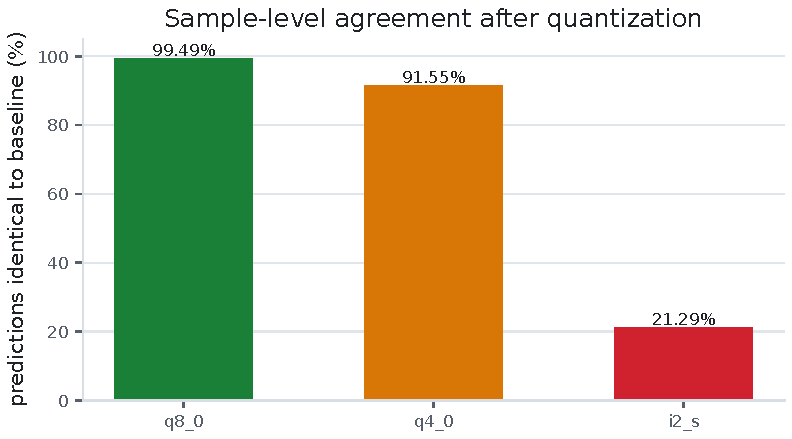
\includegraphics{figures/experiments/round3/quant_agreement.pdf}}
\caption{Sample-level agreement with the unquantized predictions for the v2 runtime.}
\label{fig:r3-quant-agreement}
\end{figure}

Two negative results complete the section. Parameter count does not predict robustness to 2-bit quantization (Spearman $-0.11$ between the \texttt{i2\_s} delta and the parameter count), and training loss does not predict held-out quality (Spearman $+0.14$). At this scale the only reliable signal is the comparison itself: measure the quantized export against the unquantized one, on the same samples, and report the agreement rather than the aggregate.

\begin{figure}[tbp]
\centering
\fitfigure{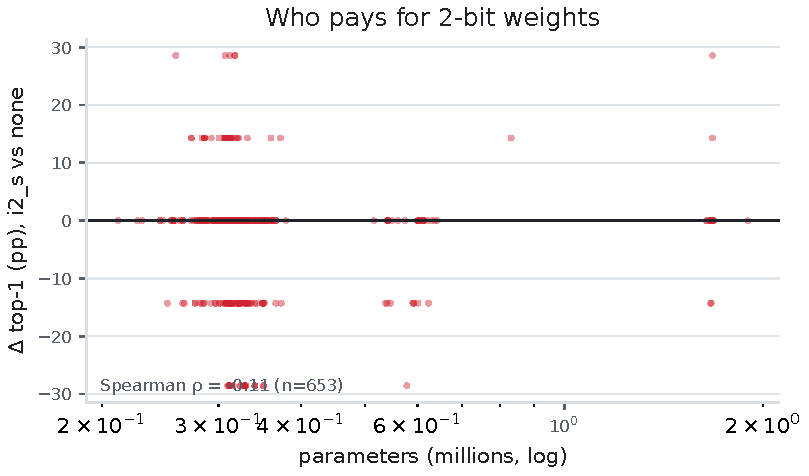
\includegraphics{figures/experiments/round3/quant_delta_vs_params.pdf}}
\caption{2-bit accuracy delta against parameter count.}
\label{fig:r3-quant-params}
\end{figure}
\begin{figure}[tbp]
\centering
\fitfigure{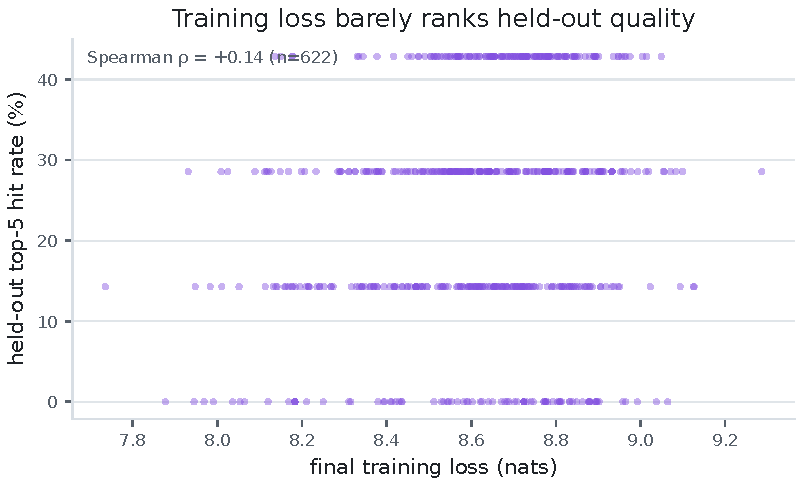
\includegraphics{figures/experiments/round3/train_vs_inference.pdf}}
\caption{Final training loss against held-out top-5 hit rate for the MLM pairs.}
\label{fig:r3-train-inference}
\end{figure}

\subsection{Reliability and failure taxonomy}
\label{sec:r3-reliability}

Training is reliable: $1{,}643$ of $1{,}653$ runs succeed ($0.6\%$ failure rate). All ten failures are hybrid pairs that contain \texttt{engram}; eight exit with code 1 and two with code 134 (SIGABRT), and no other family fails. The failure is structural rather than random---\texttt{engram} is the only mixer with an external memory bank, and ten of the fifty-three pairs that use it crash while the other forty-three train---which is why the atlas still contains every cell: the ten failed pairs are present in the population table but absent from the loss and inference analyses.

The rest of the pipeline is healthier than in Round~2. The Transformers export never fails ($4{,}686$ records, all OK), inference evaluation fails once (a \texttt{pape\_efficient} run), and the only systemic problem is the deploy stage excluded above. The stage ledger (Figure~\ref{fig:r3-stage-status}) makes the asymmetry visible: training and export are almost entirely green, inference is green with one red row, and deploy is the only stage with a large red block.

\begin{figure}[tbp]
\centering
\fitfigure{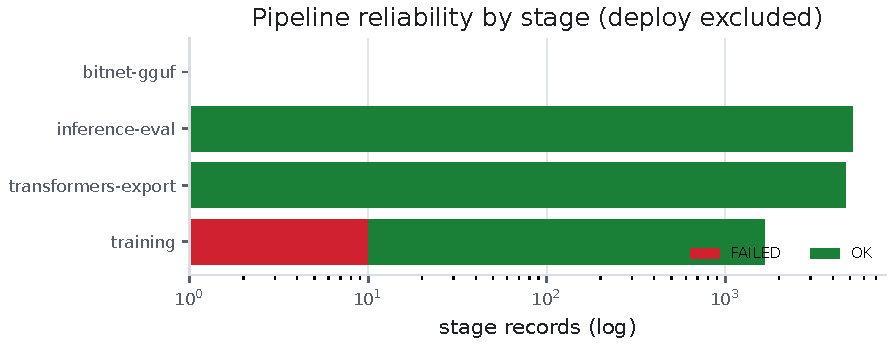
\includegraphics{figures/experiments/round3/stage_status.pdf}}
\caption{Pipeline status per stage, deploy excluded.}
\label{fig:r3-stage-status}
\end{figure}

\subsection{Correlations}

Figure~\ref{fig:r3-correlation} is the Spearman matrix of the measured features over the $1{,}431$ pairs. The strongest non-trivial correlations are the ones that describe the schedule rather than the architecture: training time grows with the number of epochs ($+0.74$), throughput is almost the inverse of step time ($-0.95$) and mean loss falls as the schedule lengthens ($-0.76$). The parameter count correlates moderately with loss ($-0.42$) and gradient magnitude ($+0.47$) and weakly with wall time ($+0.23$), the quantitative form of the weak cost law of the previous section.

\begin{figure}[tbp]
\centering
\fitfigure{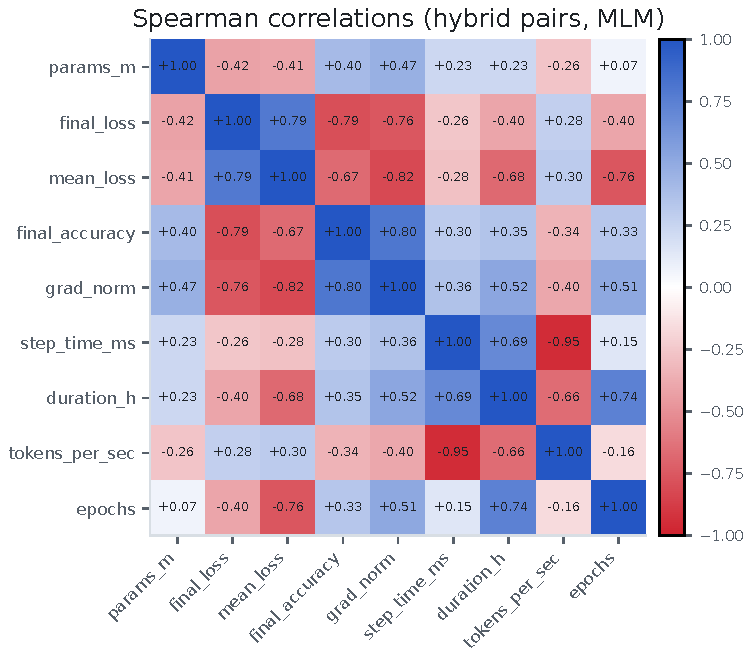
\includegraphics{figures/experiments/round3/correlation.pdf}}
\caption{Spearman correlations of the measured features over the hybrid pairs.}
\label{fig:r3-correlation}
\end{figure}

\subsection{Summary of findings}

\begin{enumerate}[leftmargin=1.4em,itemsep=2pt]
\item The complete atlas is measurable in one week of a single CPU host: $1{,}653$ runs, $20.5$ million steps, $3{,}668$ hours, a $0.6\%$ training failure rate and no NaN step.
\item The mixer stack dominates the design space. The best pair reaches $7.736$ nats and the worst $9.70$, while the optimizer, normalization and positional-encoding ablations move the loss by less than the pair spread.
\item Size helps but does not decide: the rank correlation between parameters and loss is $-0.42$, and the cheapest mixers sit on both sides of the median.
\item Learning is fast and the ranking is decided early: the median pair reaches 90\% of its loss drop at $41\%$ of the schedule, and the top ten separate from the population in the first 15\%.
\item Gradient pressure is stable and block-specific: the head ($3.66$), attention ($2.12$) and FFN ($0.71$) dominate, the coefficients of variation of the active blocks stay below 0.35, and the block ordering is constant across the campaign.
\item Clipping is routine, not exceptional: the median clip ratio is $1.04$ and $51.6\%$ of the runs clip on average, which changes the reading of the gradient norms to post-clip quantities.
\item Training time is almost independent of the parameter count at a fixed schedule (log-log exponent $0.25$, $R^2=0.06$): the number of steps dominates, and the hybrid pairs absorb $90.0\%$ of the $3{,}668$ hours.
\item Quantization at 8 and 4 bits is essentially lossless in the \texttt{v2} runtime ($99.5\%$ and $91.8\%$ sample agreement), while 2-bit weights change the model qualitatively ($20.8\%$ agreement, $-2.03$ points of top-1).
\item The pipeline is reliable except for the deploy stage, whose configuration-payload bug is documented and excluded; the Transformers export and evaluation paths are clean.
\item The round inherits the central warning of Round~2: training loss and held-out quality are almost uncorrelated ($+0.14$), so the atlas should be read as a map of learning speed and stability, not as a leaderboard.
\end{enumerate}

\subsection{Reproducing this annex}

The annex is generated by four scripts under \texttt{experimentos/3/report/}, in order:

\begin{verbatim}
python experimentos/to_csv.py 3                       # flat CSV export
python experimentos/3/report/build_data.py            # master/epochs/inference
python experimentos/3/report/make_paper_figures.py    # PDF/SVG, both languages
python experimentos/3/report/make_report.py           # stats + this annex
\end{verbatim}

\texttt{build\_data.py} streams the 6.6\,GB per-step log once (about ten minutes) and caches every aggregate; the other three scripts run in seconds. \texttt{make\_report.py} writes \texttt{out/stats.json} with every number quoted above, so any claim can be traced back to the CSV that produced it.
